\documentclass[12pt]{article}
\usepackage[utf8]{inputenc}
\usepackage[T1]{fontenc}
\usepackage{graphicx}
\usepackage{subcaption}
\usepackage{amsmath}
\usepackage{fancyhdr}
\usepackage{geometry}
\usepackage[english]{babel}
\usepackage{csquotes}
\usepackage{hyperref}
\usepackage{url}
\usepackage{listings}
\usepackage{float}
\usepackage{booktabs}
\usepackage{array}
\usepackage{tikz}
\usetikzlibrary{
    shapes.geometric, shapes.misc,
    arrows.meta, positioning, fit,
    backgrounds, calc, decorations.pathreplacing,
    automata
}
\usepackage{setspace}

\lstset{
    language=C,
    basicstyle=\ttfamily\small,
    numberstyle=\tiny,
    frame=single,
    breaklines=true,
}

% ── TikZ styles ────────────────────────────────────────────────────────────────
\tikzset{
  comp/.style={rectangle, draw, rounded corners=3pt,
               minimum width=2.8cm, minimum height=0.75cm,
               align=center, font=\small},
  hw/.style={comp, fill=gray!20},
  driver/.style={comp, fill=blue!15},
  service/.style={comp, fill=green!15},
  task/.style={comp, fill=orange!20},
  app/.style={comp, fill=yellow!20},
  arr/.style={-Stealth, thick},
  biarr/.style={Stealth-Stealth, thick},
  layer/.style={rectangle, draw, minimum height=0.9cm,
                align=center, font=\small\bfseries},
  cls/.style={rectangle, draw, font=\small, text width=2.8cm,
              minimum width=3.0cm, inner sep=3pt},
  hdr/.style={cls, fill=gray!10, align=center, font=\small\bfseries},
  uses/.style={-Stealth, dashed, thick},
  impl/.style={-Stealth, thick},
  flowstart/.style={ellipse, draw, fill=gray!20,
                    minimum width=2.5cm, minimum height=0.7cm,
                    align=center, font=\small},
  flowstep/.style={rectangle, draw, fill=blue!10,
                   minimum width=3.8cm, minimum height=0.7cm,
                   align=center, font=\small},
  flowdec/.style={diamond, draw, fill=yellow!20, aspect=2.8,
                  align=center, font=\small},
  flowres/.style={rectangle, draw, fill=green!15,
                  minimum width=3.5cm, minimum height=0.7cm,
                  align=center, font=\small},
  flowresR/.style={rectangle, draw, fill=red!15,
                   minimum width=3.5cm, minimum height=0.7cm,
                   align=center, font=\small},
  state/.style={circle, draw, fill=blue!10, minimum size=1.5cm,
                align=center, font=\small\bfseries},
}
% ───────────────────────────────────────────────────────────────────────────────

\linespread{1.25}
\setlength{\parindent}{0.8cm}
\setlength{\parskip}{0em}
\renewcommand{\headrulewidth}{0pt}
\geometry{a4paper, portrait, margin=1in}
\setlength{\headheight}{14.49998pt}

\begin{document}
\begin{titlepage}
   \begin{center}
    \textsc{\large Ministry of Education of Republic of Moldova}\\[0.5cm]
    \textsc{\large Technical University of Moldova}\\[0.5cm]
    \textsc{\large Faculty of Computers, Informatics and Microelectronics}\\[0.5cm]
    \textsc{\large Software Engineering Department}\\[1.2cm]

    \vspace{25mm}

    {\LARGE \textbf{\textsc{Embedded Systems}}}\\[0.5cm]
    \textsc{\large Laboratory No. 1.4}\\[0.5cm]

    \newcommand{\HRule}{\rule{\linewidth}{0.5mm}}
    \vspace{80mm}

    \begin{minipage}[t]{0.4\textwidth}
    \begin{flushleft} \large
    \emph{Author:} \\
    Vladimir \textsc{Vitcovschii}\\
    std. gr. FAF-231
    \end{flushleft}
    \end{minipage}
    ~
    \begin{minipage}[t]{0.4\textwidth}
    \begin{flushright} \large
    \end{flushright}
    \end{minipage}\\[3cm]

    \vspace{5mm}
    \large Chișinău 2026\\[0.5cm]

    \vfill
    \end{center}
\end{titlepage}

\clearpage
\tableofcontents
\clearpage

\setcounter{page}{2}
\pagestyle{fancy}
\fancyhf{}
\rhead{\thepage}
\lhead{FAF-231 Vitcovschii Vladimir; Laboratory Work No. 1.4}

% ─────────────────────────────────────────────────────────────────────────────
\section{The Purpose of the Work}
% ─────────────────────────────────────────────────────────────────────────────

The purpose of this laboratory work is to develop a multitasking embedded application using FreeRTOS on an ATmega2560 microcontroller, replacing the bare-metal cooperative scheduler from Laboratory~1.3 with preemptive real-time tasks. The focus is on correct inter-task synchronisation using binary semaphores and mutexes, task-level code reuse across bare-metal and RTOS execution models, and the practical comparison of both approaches for the same button-monitoring application.

% ─────────────────────────────────────────────────────────────────────────────
\section{Objectives of the Work}
% ─────────────────────────────────────────────────────────────────────────────

The task requires porting the bare-metal button-press monitor from Lab~1.3 to a FreeRTOS-based multitasking application on an ATmega2560, implementing at least three concurrent tasks:
\begin{itemize}
  \item \textbf{Task~1 — Button Detector}: Detect button presses using a non-blocking FSM, classify each press as short (\(<\)500\,ms) or long (\(\geq\)500\,ms), light the corresponding LED, and signal Task~2 via a binary semaphore.
  \item \textbf{Task~2 — Press Counter / LED Blinker}: Block on the semaphore from Task~1; on each signal, consume the press result, record statistics under mutex protection, and drive a yellow LED blink sequence (5 blinks for short, 10 for long).
  \item \textbf{Task~3 — Status Reporter}: Every 10\,s, acquire the statistics mutex, snapshot and reset the counters, and emit a formatted report via \texttt{printf} over serial STDIO.
  \item Reuse the core task logic (\texttt{TaskButtonMeasure}, \texttt{TaskPressStats}) from Lab~1.3 without modification, wrapping them in FreeRTOS task functions.
  \item Replace \texttt{cli()}/\texttt{sei()} critical sections with FreeRTOS mutex-based synchronisation for protecting shared \texttt{PressData} statistics.
  \item Ensure all tasks run concurrently without blocking or data corruption.
\end{itemize}

% ─────────────────────────────────────────────────────────────────────────────
\section{Domain Analysis}
% ─────────────────────────────────────────────────────────────────────────────

\subsection{FreeRTOS on AVR}

FreeRTOS is a widely-used real-time operating system kernel for embedded microcontrollers. On AVR targets, the port uses a hardware timer (Timer1 or Timer3, depending on the port) to generate the RTOS tick interrupt, which drives the scheduler. Each task has its own stack and execution context; the kernel performs context switches at each tick and whenever a task voluntarily blocks (e.g., on a semaphore or delay).

The FreeRTOS Arduino library (\texttt{feilipu/FreeRTOS}) provides a drop-in integration for the Arduino framework. Tasks are created with \texttt{xTaskCreate()}, which allocates a stack on the heap. The scheduler is started with \texttt{vTaskStartScheduler()}, which never returns — the \texttt{loop()} function becomes unreachable. \cite{freertos_sem}

\subsection{Binary Semaphores}

A binary semaphore is the lightest FreeRTOS synchronisation primitive. It has two states: \emph{available} (given) and \emph{taken}. A producer task calls \texttt{xSemaphoreGive()} to signal an event; a consumer task calls \texttt{xSemaphoreTake()} to wait for it. If the semaphore is not available, the consumer blocks (suspends) and consumes zero CPU until the producer signals.

In this application, the binary semaphore \texttt{xPressSemaphore} replaces the producer-before-consumer ordering guarantee that the bare-metal scheduler provided implicitly through registration order. The RTOS version is more robust: Task~2 blocks until Task~1 has actually produced a result, regardless of scheduling order. \cite{freertos_sem}

\subsection{Mutexes}

A mutex (mutual exclusion) is a semaphore with priority inheritance. When a low-priority task holds a mutex and a higher-priority task attempts to take it, the kernel temporarily raises the holder's priority to prevent priority inversion. In this application, \texttt{xStatsMutex} protects the \texttt{PressStats} structure from concurrent access by Task~2 (writer) and Task~3 (reader/resetter). \cite{freertos_mutex}

\subsection{Comparison: Bare-Metal vs.\ RTOS Synchronisation}

\begin{table}[H]
\centering
\begin{tabular}{@{}p{3.5cm}p{4.8cm}p{4.8cm}@{}}
\toprule
\textbf{Aspect} & \textbf{Bare-Metal (Lab 1.3)} & \textbf{FreeRTOS (Lab 1.4)} \\
\midrule
Task ordering       & Registration order in ISR     & Semaphore-driven event signalling \\
Stats protection    & \texttt{cli()}/\texttt{sei()} critical section & \texttt{xStatsMutex} with priority inheritance \\
Serial I/O safety   & Flag + main-loop drain        & Direct \texttt{printf} in task context (safe) \\
Timer usage         & Timer1 CTC for scheduler tick  & Timer used by FreeRTOS kernel \\
CPU idle behaviour  & Busy-loop in \texttt{loop()}   & Idle task runs (optional low-power) \\
\bottomrule
\end{tabular}
\caption{Bare-Metal vs.\ FreeRTOS Synchronisation}
\label{tab:comparison}
\end{table}

\subsection{Technology Stack}

\begin{table}[H]
\centering
\begin{tabular}{@{}lll@{}}
\toprule
\textbf{Layer} & \textbf{Technology} & \textbf{Details} \\
\midrule
Hardware Platform    & Arduino Mega 2560  & ATmega2560, 16\,MHz, 5\,V \\
Build System         & PlatformIO         & \texttt{atmelavr} platform, Arduino framework \\
Programming Language & C++                & AVR-GCC toolchain \\
RTOS                 & FreeRTOS 10.5.1    & \texttt{feilipu/FreeRTOS} Arduino library \\
STDIO Hook           & AVR-libc           & \texttt{fdev\_setup\_stream} → \texttt{SerialStream} \\
Serial Communication & UART0              & 9600\,baud, 8N1 \\
Simulation           & Wokwi / SimulIDE   & Real-time circuit and firmware simulation \\
\bottomrule
\end{tabular}
\caption{Technology Stack}
\label{tab:techstack}
\end{table}

\subsection{System Elements}

\begin{itemize}
  \item \textbf{Arduino Mega 2560 (ATmega2560)}: 256\,KB flash, 8\,KB SRAM, 16\,MHz. FreeRTOS uses one hardware timer for its tick; remaining timers are free for application use.
  \item \textbf{Push Button (D2)}: Momentary tactile switch connected between D2 and GND. Configured as \texttt{INPUT\_PULLUP}; reads LOW when pressed.
  \item \textbf{Green LED (D12)}: Indicates a short press (\(<\)500\,ms). 220\,\(\Omega\) current-limiting resistor.
  \item \textbf{Red LED (D11)}: Indicates a long press (\(\geq\)500\,ms). Same resistor topology.
  \item \textbf{Yellow LED (D10)}: Blinks 5 times for a short press and 10 times for a long press.
  \item \textbf{PlatformIO}: Build system with \texttt{env:mega} environment defining \texttt{-D USE\_FREERTOS -D ACTIVE\_LAB=4}. \cite{pio}
\end{itemize}

% ─────────────────────────────────────────────────────────────────────────────
\section{Design}
% ─────────────────────────────────────────────────────────────────────────────

\subsection{Architectural Design}

% ── Mermaid source (render externally and save as images/lab4_component.png) ──
% ```mermaid
% graph TD
%     subgraph APP["APP Layer"]
%         MainLab4["MainLab4<br/>SetupLab4 / LoopLab4"]
%     end
%     subgraph TASKS["TASKS Layer"]
%         T1["TaskButtonMeasureRtosFunc<br/>20 ms periodic"]
%         T2["TaskPressStatsRtosFunc<br/>event-driven"]
%         T3["TaskReportRtosFunc<br/>10 s periodic"]
%     end
%     subgraph SRV["SRV Layer"]
%         PD["PressData<br/>volatile shared data"]
%         STDIO["StdioRedirect"]
%         SYNC["SyncObjects<br/>xPressSemaphore<br/>xStatsMutex"]
%     end
%     subgraph ECAL["ECAL Layer"]
%         BD["ButtonDriver"]
%         LD["LedDriver"]
%         SS["SerialStream<br/>IStream"]
%     end
%     subgraph HW["HW Layer"]
%         MCU["ATmega2560"]
%         BTN["Button D2"]
%         LEDS["LEDs D10,D11,D12"]
%         UART["UART0"]
%     end
%     MainLab4 --> T1
%     MainLab4 --> T2
%     MainLab4 --> T3
%     T1 -->|SetPressResult| PD
%     T1 -->|xSemaphoreGive| SYNC
%     T2 -->|xSemaphoreTake| SYNC
%     T2 -->|RecordPress| PD
%     T2 -->|xStatsMutex| SYNC
%     T3 -->|GetStats/Reset| PD
%     T3 -->|xStatsMutex| SYNC
%     T3 -->|printf| STDIO
%     T1 --> BD
%     T1 --> LD
%     T2 --> LD
%     STDIO --> SS
%     BD --> MCU
%     LD --> MCU
%     SS --> UART
%     MCU --- BTN
%     MCU --- LEDS
%     MCU --- UART
% ```

\begin{figure}[H]
\centering
\includegraphics[width=0.85\textwidth]{images/lab4_component.png}
\caption{Component Diagram — FreeRTOS Button Monitor}
\label{fig:component}
\end{figure}

Table~\ref{tab:components} summarises the role of each component.

\begin{table}[H]
\centering
\begin{tabular}{@{}p{3.6cm}p{2.8cm}p{6.0cm}@{}}
\toprule
\textbf{Component} & \textbf{Role} & \textbf{Interface / Key Operation} \\
\midrule
Button (D2)                  & User input        & Active-LOW; \texttt{INPUT\_PULLUP} \\
ButtonDriver                 & GPIO abstraction   & \texttt{InitializeButton}, \texttt{ReadButtonRaw} \\
LedDriver                    & GPIO abstraction   & \texttt{InitializeLed}, \texttt{SetLedState} \\
SerialStream                 & UART adapter       & \texttt{IStream} over \texttt{HardwareSerial} \\
PressData                    & Shared data        & \texttt{volatile} flag + 32-bit duration; stats struct \\
SyncObjects                  & RTOS sync          & \texttt{xPressSemaphore} (binary), \texttt{xStatsMutex} \\
TaskButtonMeasureRtosFunc    & Producer task      & Wraps \texttt{TaskButtonMeasure}; gives semaphore \\
TaskPressStatsRtosFunc       & Consumer task      & Blocks on semaphore; records stats under mutex \\
TaskReportRtosFunc           & Reporter task      & 10\,s period; snapshots stats under mutex \\
StdioRedirect                & RTE glue           & \texttt{initStdio(IStream*)} \\
MainLab4                     & Entry point        & Creates sync objects, tasks; starts scheduler \\
\bottomrule
\end{tabular}
\caption{Software Component Roles}
\label{tab:components}
\end{table}

\subsection{Interface Design — Layered Architecture}

\begin{figure}[H]
\centering
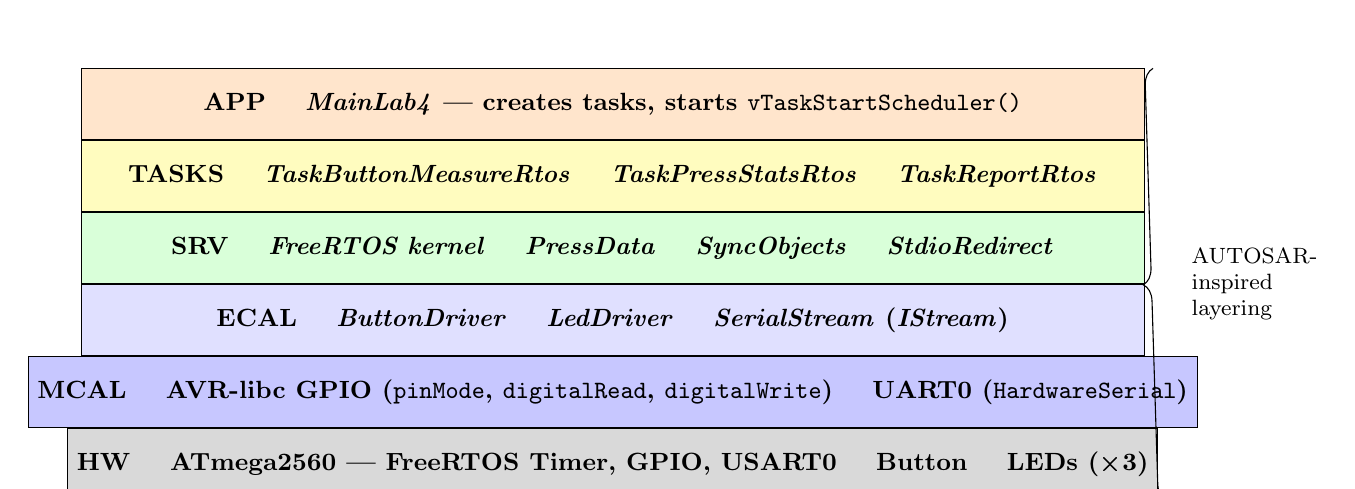
\begin{tikzpicture}[node distance=0pt]

  \def\LW{13.5cm}

  \node[layer, minimum width=\LW, fill=orange!20] (app)
    {\textbf{APP} \quad \textit{MainLab4} — creates tasks, starts \texttt{vTaskStartScheduler()}};

  \node[layer, minimum width=\LW, fill=yellow!25, below=of app] (tasks)
    {\textbf{TASKS} \quad \textit{TaskButtonMeasureRtos} \quad \textit{TaskPressStatsRtos} \quad \textit{TaskReportRtos}};

  \node[layer, minimum width=\LW, fill=green!15, below=of tasks] (srv)
    {\textbf{SRV} \quad \textit{FreeRTOS kernel} \quad \textit{PressData} \quad \textit{SyncObjects} \quad \textit{StdioRedirect}};

  \node[layer, minimum width=\LW, fill=blue!12, below=of srv] (ecal)
    {\textbf{ECAL} \quad \textit{ButtonDriver} \quad \textit{LedDriver} \quad \textit{SerialStream} (\textit{IStream})};

  \node[layer, minimum width=\LW, fill=blue!22, below=of ecal] (mcal)
    {\textbf{MCAL} \quad AVR-libc GPIO (\texttt{pinMode}, \texttt{digitalRead}, \texttt{digitalWrite}) \quad UART0 (\texttt{HardwareSerial})};

  \node[layer, minimum width=\LW, fill=gray!30, below=of mcal] (hw)
    {\textbf{HW} \quad ATmega2560 — FreeRTOS Timer, GPIO, USART0 \quad Button \quad LEDs (×3)};

  \draw[decorate, decoration={brace, amplitude=6pt, mirror}]
    ([xshift=3pt]app.north east) -- ([xshift=3pt]hw.south east)
    node[midway, right=8pt, font=\footnotesize, align=left]
    {AUTOSAR-\\inspired\\layering};

\end{tikzpicture}
\caption{Layered Software Architecture}
\label{fig:layers}
\end{figure}

\begin{itemize}
  \item \textbf{APP}: \texttt{MainLab4} wires all components, creates the two synchronisation objects (\texttt{xPressSemaphore}, \texttt{xStatsMutex}), creates three FreeRTOS tasks, prints the welcome message, and starts the scheduler. \texttt{LoopLab4()} is empty — never reached.
  \item \textbf{TASKS}: Three FreeRTOS task functions wrapping the reused bare-metal task logic. Each runs in its own execution context with its own stack.
  \item \textbf{SRV}: The FreeRTOS kernel provides tick-based scheduling, semaphores, mutexes, and \texttt{vTaskDelayUntil}. \texttt{PressData} is the shared data module. \texttt{SyncObjects.h} declares the extern handles. \texttt{StdioRedirect} connects \texttt{printf} to \texttt{SerialStream}.
  \item \textbf{ECAL}: Hardware-agnostic driver wrappers reused from Lab~1.3.
  \item \textbf{MCAL}: Arduino framework register-level abstractions.
  \item \textbf{HW}: Physical devices. FreeRTOS owns one hardware timer for the tick interrupt.
\end{itemize}

\subsection{Software Module Design}

% ── Mermaid source (render externally and save as images/lab4_modules.png) ──
% ```mermaid
% classDiagram
%     class IStream {
%         <<interface>>
%         +write(char c)*
%         +read() char*
%         +available() bool*
%     }
%     class SerialStream {
%         +begin(unsigned long baud)
%         +write(char c)
%         +read() char
%         +available() bool
%     }
%     class ButtonDriver {
%         +InitializeButton(uint8_t pin)
%         +ReadButtonRaw(uint8_t pin) bool
%     }
%     class LedDriver {
%         +InitializeLed(int pin)
%         +SetLedState(int pin, bool on)
%     }
%     class PressData {
%         -PressReady : volatile bool
%         -LastDurationMs : volatile uint32_t
%         -Stats : PressStats
%         +SetPressResult(uint32_t ms)
%         +HasPressResult() bool
%         +ConsumePressResult(uint32_t* ms) bool
%         +RecordPress(uint32_t ms)
%         +GetStats() PressStats
%         +ResetStats()
%     }
%     class SyncObjects {
%         +xPressSemaphore : SemaphoreHandle_t
%         +xStatsMutex : SemaphoreHandle_t
%     }
%     class TaskButtonMeasure {
%         -State : ButtonState
%         -PressStartMs : uint32_t
%         +TaskButtonMeasureInit()
%         +TaskButtonMeasure()
%     }
%     class TaskPressStats {
%         -BlinkRemaining : uint8_t
%         +TaskPressStatsInit()
%         +TaskPressStats()
%     }
%     class TaskButtonMeasureRtos {
%         +TaskButtonMeasureRtosFunc(void*)
%     }
%     class TaskPressStatsRtos {
%         +TaskPressStatsRtosFunc(void*)
%     }
%     class TaskReportRtos {
%         +TaskReportRtosFunc(void*)
%     }
%     SerialStream ..|> IStream
%     TaskButtonMeasureRtos --> TaskButtonMeasure : reuses
%     TaskButtonMeasureRtos --> PressData : SetPressResult
%     TaskButtonMeasureRtos --> SyncObjects : xSemaphoreGive
%     TaskPressStatsRtos --> TaskPressStats : reuses
%     TaskPressStatsRtos --> PressData : ConsumePressResult, RecordPress
%     TaskPressStatsRtos --> SyncObjects : xSemaphoreTake
%     TaskReportRtos --> PressData : GetStats, ResetStats
%     TaskReportRtos --> SyncObjects : xStatsMutex
%     TaskButtonMeasure --> ButtonDriver
%     TaskButtonMeasure --> LedDriver
%     TaskPressStats --> LedDriver
% ```

\begin{figure}[H]
\centering
\includegraphics[width=0.85\textwidth]{images/lab4_modules.png}
\caption{Software Module Diagram}
\label{fig:modules}
\end{figure}

\subsection{FreeRTOS Task Synchronisation Diagram}

% ── Mermaid source (render externally and save as images/lab4_sequence.png) ──
% ```mermaid
% sequenceDiagram
%     participant T1 as Task1: ButtonMeasure<br/>(20ms periodic)
%     participant SEM as xPressSemaphore<br/>(binary)
%     participant T2 as Task2: PressStats<br/>(event-driven)
%     participant MTX as xStatsMutex
%     participant PD as PressData
%     participant T3 as Task3: Report<br/>(10s periodic)
%
%     Note over T1: Button released
%     T1->>PD: SetPressResult(duration)
%     T1->>SEM: xSemaphoreGive()
%     SEM-->>T2: unblocks
%     T2->>PD: ConsumePressResult(&dur)
%     T2->>MTX: xSemaphoreTake()
%     T2->>PD: RecordPress(dur)
%     T2->>MTX: xSemaphoreGive()
%     T2->>T2: TaskPressStats() [blink LED]
%
%     Note over T3: 10s elapsed
%     T3->>MTX: xSemaphoreTake()
%     T3->>PD: GetStats() + ResetStats()
%     T3->>MTX: xSemaphoreGive()
%     T3->>T3: printf() report
% ```

\begin{figure}[H]
\centering
\includegraphics[width=0.85\textwidth]{images/lab4_sequence.png}
\caption{FreeRTOS Task Synchronisation Sequence}
\label{fig:sequence}
\end{figure}

The synchronisation architecture:
\begin{itemize}
  \item \textbf{xPressSemaphore} (binary): Task~1 gives after a press result is deposited; Task~2 blocks on take with \texttt{portMAX\_DELAY} — zero CPU while waiting.
  \item \textbf{xStatsMutex}: Protects the \texttt{PressStats} structure. Task~2 acquires it to call \texttt{RecordPress()}, Task~3 acquires it to snapshot \texttt{GetStats()} and call \texttt{ResetStats()}.
  \item All three tasks have equal priority (1), so the RTOS round-robins among ready tasks at each tick.
\end{itemize}

\subsection{TaskButtonMeasure — State Machine (Reused)}

\begin{figure}[H]
\centering
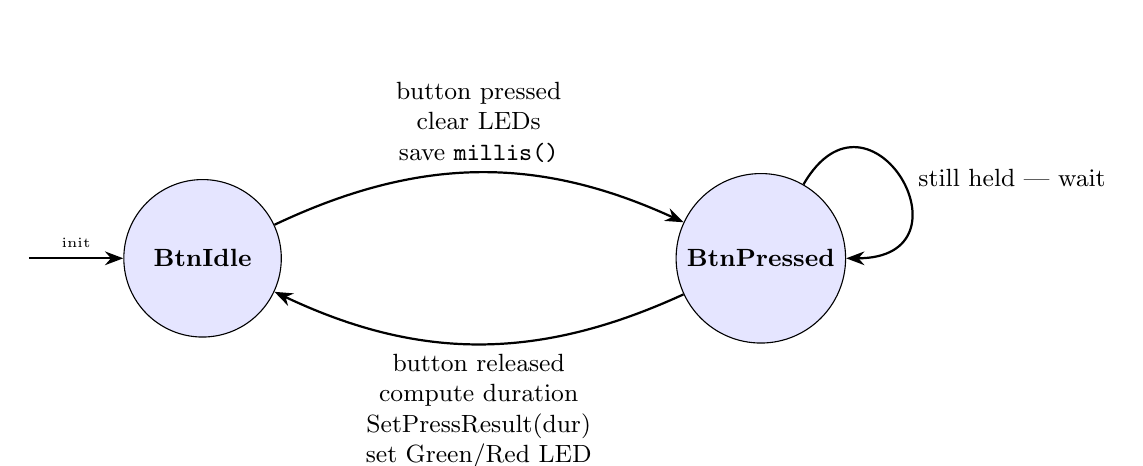
\begin{tikzpicture}[
  state/.style={circle, draw, fill=blue!10, minimum size=2.0cm,
                align=center, font=\small\bfseries},
  arr/.style={-Stealth, thick},
  node distance=5.0cm
]
  \node[state] (idle)    {BtnIdle};
  \node[state, right=of idle] (pressed) {BtnPressed};

  \draw[arr, bend left=25] (idle) to
    node[above, font=\small, align=center]
      {button pressed\\clear LEDs\\save \texttt{millis()}}
    (pressed);

  \draw[arr, bend left=25] (pressed) to
    node[below, font=\small, align=center]
      {button released\\compute duration\\SetPressResult(dur)\\set Green/Red LED}
    (idle);

  \draw[arr] (pressed.60) to[out=60, in=0, looseness=4]
    node[right, font=\small, xshift=3pt]{still held — wait}
    (pressed.0);

  \draw[arr] ($(idle.west)+(-1.2,0)$) -- (idle.west)
    node[midway, above, font=\tiny]{init};

\end{tikzpicture}
\caption{TaskButtonMeasure — Finite State Machine (reused from Lab~1.3)}
\label{fig:fsm}
\end{figure}

The FSM is identical to Lab~1.3. In the FreeRTOS context, the wrapper function \texttt{TaskButtonMeasureRtosFunc} calls \texttt{TaskButtonMeasure()} every 20\,ms via \texttt{vTaskDelayUntil}. The key difference is what happens after \texttt{SetPressResult()}: the wrapper checks whether a new result appeared and calls \texttt{xSemaphoreGive(xPressSemaphore)} to unblock Task~2.

\subsection{Electronic Design}

\begin{figure}[H]
\centering
\begin{tikzpicture}[
  blk/.style={rectangle, draw, minimum height=1.4cm, align=center, font=\small},
  mcu/.style={blk, fill=gray!15, minimum width=3.0cm, minimum height=7.5cm},
  ledb/.style={blk, fill=green!20, minimum width=2.0cm, minimum height=0.75cm},
  ledr/.style={blk, fill=red!20,   minimum width=2.0cm, minimum height=0.75cm},
  ledy/.style={blk, fill=yellow!30, minimum width=2.0cm, minimum height=0.75cm},
  btnb/.style={blk, fill=gray!20,  minimum width=2.0cm, minimum height=0.75cm},
  bus/.style={-Stealth, thick},
  lbl/.style={font=\tiny, midway},
]

  \node[mcu] (mcu) {Arduino Mega\\2560\\[4pt]
    \tiny D2 ← Button\\[2pt]
    D10 → Yellow LED\\D11 → Red LED\\D12 → Green LED\\[2pt]
    UART0 TX/RX};

  \node[btnb, left=2.8cm of mcu, yshift=2.0cm] (btn)
    {Push Button\\{\tiny D2, INPUT\_PULLUP}};

  \node[ledb, right=2.8cm of mcu, yshift=2.2cm] (gled)
    {Green LED\\{\tiny D12, 220\,Ω}};

  \node[ledr, right=2.8cm of mcu, yshift=1.0cm] (rled)
    {Red LED\\{\tiny D11, 220\,Ω}};

  \node[ledy, right=2.8cm of mcu, yshift=-0.2cm] (yled)
    {Yellow LED\\{\tiny D10, 220\,Ω}};

  \node[blk, fill=blue!10, minimum width=2.0cm, minimum height=0.75cm, right=2.8cm of mcu, yshift=-1.6cm] (ser)
    {PC Terminal\\{\tiny UART 9600 baud}};

  \draw[bus] (btn.east) -- node[lbl, above]{D2} (mcu.west |- btn.east);

  \draw[bus] (mcu.east |- gled.west) -- node[lbl, above]{D12} (gled.west);
  \draw[bus] (mcu.east |- rled.west) -- node[lbl, above]{D11} (rled.west);
  \draw[bus] (mcu.east |- yled.west) -- node[lbl, above]{D10} (yled.west);
  \draw[bus, Stealth-Stealth] (mcu.east |- ser.west) --
    node[lbl, above]{TX/RX} (ser.west);

  \foreach \led in {gled, rled, yled}
    \draw[thick] (\led.east) -- ++(0.4,0) node[right, font=\tiny]{GND};

  \draw[thick] (btn.west) -- ++(-0.4,0) node[left, font=\tiny]{GND};

\end{tikzpicture}
\caption{Electronic Design — Pin Connection Diagram}
\label{fig:elec}
\end{figure}

The hardware configuration is identical to Lab~1.3 except that the target board is an Arduino Mega~2560 (ATmega2560). The pin assignments remain the same:
\begin{itemize}
  \item \textbf{Button (D2)}: Connected between D2 and GND. \texttt{INPUT\_PULLUP}; active-LOW.
  \item \textbf{Green LED (D12)}: Short press indicator. 220\,\(\Omega\) series resistor.
  \item \textbf{Red LED (D11)}: Long press indicator. Same resistor topology.
  \item \textbf{Yellow LED (D10)}: Blink acknowledgement (5 for short, 10 for long).
  \item \textbf{UART0 (TX/RX)}: 9600\,baud serial connection for the 10\,s report.
\end{itemize}

% ─────────────────────────────────────────────────────────────────────────────
\section{Implementation}
% ─────────────────────────────────────────────────────────────────────────────

\subsection{Project Structure}

\begin{table}[H]
\centering
\begin{tabular}{@{}lp{8.2cm}@{}}
\toprule
\textbf{File} & \textbf{Purpose} \\
\midrule
\texttt{src/main.cpp}
  & Lab selector; dispatches \texttt{setup()}/\texttt{loop()} based on \texttt{ACTIVE\_LAB} \\
\texttt{src/labs/lab4/MainLab4.cpp}
  & Creates sync objects and FreeRTOS tasks; calls \texttt{vTaskStartScheduler()} \\
\texttt{src/labs/lab4/TaskButtonMeasureRtos.cpp}
  & 20\,ms periodic FreeRTOS wrapper around \texttt{TaskButtonMeasure()} \\
\texttt{src/labs/lab4/TaskPressStatsRtos.cpp}
  & Event-driven FreeRTOS wrapper; blocks on \texttt{xPressSemaphore} \\
\texttt{src/labs/lab4/TaskReportRtos.cpp}
  & 10\,s periodic report via \texttt{printf\_P} under mutex protection \\
\texttt{src/labs/lab3/TaskButtonMeasure.cpp}
  & Reused: non-blocking button FSM \\
\texttt{src/labs/lab3/TaskPressStats.cpp}
  & Reused: press consumer + yellow LED blink FSM \\
\texttt{src/components/PressData.cpp}
  & Volatile shared data: press-ready flag, duration, stats \\
\texttt{src/components/ButtonDriver.cpp}
  & \texttt{InitializeButton} / \texttt{ReadButtonRaw} — active-LOW GPIO \\
\texttt{src/components/LedDriver.cpp}
  & \texttt{InitializeLed} / \texttt{SetLedState} — GPIO output \\
\texttt{src/components/SerialStream.cpp}
  & \texttt{IStream} implementation over \texttt{HardwareSerial} \\
\texttt{src/components/StdioRedirect.cpp}
  & \texttt{initStdio(IStream*)} via \texttt{fdev\_setup\_stream} \\
\texttt{include/labs/lab3/SyncObjects.h}
  & Declares \texttt{xPressSemaphore} and \texttt{xStatsMutex} (guarded by \texttt{USE\_FREERTOS}) \\
\texttt{include/services/PressData.h}
  & \texttt{PressStats} struct; all PressData API declarations \\
\bottomrule
\end{tabular}
\caption{Project File Structure}
\label{tab:files}
\end{table}

\subsection{PlatformIO Environment Configuration}

The FreeRTOS build is selected via the \texttt{[env:mega]} environment in \texttt{platformio.ini}:

\begin{lstlisting}
[env:mega]
platform  = atmelavr
board     = megaatmega2560
framework = arduino
lib_deps  = feilipu/FreeRTOS@^10.5.1-1
build_flags =
    -D USE_FREERTOS
    -D ACTIVE_LAB=4
\end{lstlisting}

The \texttt{-D USE\_FREERTOS} flag serves two purposes: (1) it enables \texttt{SyncObjects.h} declarations, and (2) it guards the bare-metal \texttt{ISR(TIMER1\_COMPA\_vect)} in \texttt{Scheduler.cpp} with \texttt{\#ifndef USE\_FREERTOS}, preventing a conflict with the FreeRTOS tick ISR.

\subsection{Task Setup and Scheduler Launch}

\texttt{SetupLab4()} in \texttt{MainLab4.cpp} performs the following steps:
\begin{enumerate}
  \item Initialise serial at 9600\,baud and hook STDIO via \texttt{initStdio(\&SerialIo)}.
  \item Initialise button (D2) and three LEDs (D10, D11, D12).
  \item Call \texttt{TaskButtonMeasureInit()} and \texttt{TaskPressStatsInit()} with pin numbers.
  \item Create the binary semaphore: \texttt{xPressSemaphore = xSemaphoreCreateBinary()}.
  \item Create the mutex: \texttt{xStatsMutex = xSemaphoreCreateMutex()}.
  \item Create three tasks with \texttt{xTaskCreate()}: Measure (128 words stack), Stats (128 words stack), Report (200 words stack), all at priority~1.
  \item Print four welcome-message lines via \texttt{printf}.
  \item Call \texttt{vTaskStartScheduler()} — does not return.
\end{enumerate}

\begin{lstlisting}[caption={SetupLab4 — Task creation and scheduler launch}]
void SetupLab4() {
    SerialIo.begin(9600);
    initStdio(&SerialIo);

    InitializeButton(ButtonPin);
    InitializeLed(GreenLedPin);
    InitializeLed(RedLedPin);
    InitializeLed(YellowLedPin);

    TaskButtonMeasureInit(ButtonPin, GreenLedPin, RedLedPin);
    TaskPressStatsInit(YellowLedPin);

    xPressSemaphore = xSemaphoreCreateBinary();
    xStatsMutex     = xSemaphoreCreateMutex();

    xTaskCreate(TaskButtonMeasureRtosFunc, "Measure", 128,
                nullptr, 1, nullptr);
    xTaskCreate(TaskPressStatsRtosFunc,    "Stats",   128,
                nullptr, 1, nullptr);
    xTaskCreate(TaskReportRtosFunc,        "Report",  200,
                nullptr, 1, nullptr);

    printf("Lab 3 RTOS: Button Monitor\n");
    printf("Short < 500 ms -> green\n");
    printf("Long >= 500 ms -> red\n");
    printf("Report every 10 s\n");

    vTaskStartScheduler();
}
\end{lstlisting}

\subsection{TaskButtonMeasureRtosFunc — Producer}

The producer task wraps the reused bare-metal \texttt{TaskButtonMeasure()} FSM. It checks whether a new press result has appeared by comparing the \texttt{HasPressResult()} flag before and after the call. If a new result is detected, it gives the binary semaphore to unblock Task~2.

\begin{lstlisting}[caption={TaskButtonMeasureRtosFunc — FreeRTOS producer wrapper}]
void TaskButtonMeasureRtosFunc(void* pvParameters) {
    const TickType_t RecTicks = pdMS_TO_TICKS(20);
    vTaskDelay(pdMS_TO_TICKS(1));  // 1 ms offset
    TickType_t xLastWakeTime = xTaskGetTickCount();

    for (;;) {
        bool hadPending = HasPressResult();
        TaskButtonMeasure();

        if (!hadPending && HasPressResult()) {
            xSemaphoreGive(xPressSemaphore);
        }
        vTaskDelayUntil(&xLastWakeTime, RecTicks);
    }
}
\end{lstlisting}

\subsection{TaskPressStatsRtosFunc — Consumer}

Task~2 is event-driven: it blocks on \texttt{xSemaphoreTake(xPressSemaphore, portMAX\_DELAY)} until Task~1 signals a new press. It then consumes the result, acquires \texttt{xStatsMutex} to call \texttt{RecordPress()}, and drives the yellow LED blink via the reused \texttt{TaskPressStats()} function.

\begin{lstlisting}[caption={TaskPressStatsRtosFunc — FreeRTOS consumer wrapper}]
void TaskPressStatsRtosFunc(void* pvParameters) {
    vTaskDelay(pdMS_TO_TICKS(1));  // 1 ms offset

    for (;;) {
        xSemaphoreTake(xPressSemaphore, portMAX_DELAY);

        uint32_t duration;
        if (ConsumePressResult(&duration)) {
            xSemaphoreTake(xStatsMutex, portMAX_DELAY);
            RecordPress(duration);
            xSemaphoreGive(xStatsMutex);
        }
        TaskPressStats();
    }
}
\end{lstlisting}

Note that \texttt{ConsumePressResult()} is called \emph{outside} the mutex, because the press-ready flag is only accessed by the Task~1/Task~2 pair (no third party). Only the \texttt{PressStats} accumulation (shared with Task~3) needs mutex protection.

\subsection{TaskReportRtosFunc — Reporter}

Task~3 runs periodically every 10\,s (with a 50\,ms initial offset). It acquires the mutex to atomically snapshot and reset the statistics, then emits a formatted report using \texttt{printf\_P()} with PROGMEM strings to conserve SRAM on the ATmega2560.

\begin{lstlisting}[caption={TaskReportRtosFunc — periodic reporter}]
void TaskReportRtosFunc(void* pvParameters) {
    const TickType_t RecTicks = pdMS_TO_TICKS(10000);
    vTaskDelay(pdMS_TO_TICKS(50));  // 50 ms offset
    TickType_t xLastWakeTime = xTaskGetTickCount();

    for (;;) {
        xSemaphoreTake(xStatsMutex, portMAX_DELAY);
        PressStats Stats = GetStats();
        ResetStats();
        xSemaphoreGive(xStatsMutex);

        uint32_t TotalCount = Stats.ShortPresses
                            + Stats.LongPresses;
        if (TotalCount > 0) {
            uint32_t AvgMs = Stats.TotalDurationMs / TotalCount;
            uint32_t WholeSeconds = AvgMs / 1000;
            uint32_t Decimals = (AvgMs % 1000) / 10;
            printf_P(PSTR("L: %lu, S: %lu, Avg: %lu.%02lus\n\r"),
                Stats.LongPresses, Stats.ShortPresses,
                WholeSeconds, Decimals);
        } else {
            printf_P(PSTR("L: %lu, S: %lu, Avg: 0.00s\n\r"),
                Stats.LongPresses, Stats.ShortPresses);
        }
        vTaskDelayUntil(&xLastWakeTime, RecTicks);
    }
}
\end{lstlisting}

Unlike Lab~1.3, there is no flag-plus-main-loop pattern: \texttt{printf} is safe to call directly from a FreeRTOS task context because it does not run inside an ISR.

\subsection{SyncObjects Header}

The shared synchronisation handles are declared in \texttt{SyncObjects.h}, conditionally compiled only when \texttt{USE\_FREERTOS} is defined:

\begin{lstlisting}[caption={SyncObjects.h — conditional RTOS declarations}]
#pragma once
#ifdef USE_FREERTOS
#include <Arduino_FreeRTOS.h>
#include <semphr.h>

extern SemaphoreHandle_t xPressSemaphore;
extern SemaphoreHandle_t xStatsMutex;
#endif
\end{lstlisting}

\subsection{Code Reuse from Lab~1.3}

The following modules are reused without any modification:
\begin{itemize}
  \item \texttt{TaskButtonMeasure.cpp} — the non-blocking button FSM.
  \item \texttt{TaskPressStats.cpp} — the press consumer and yellow LED blink FSM.
  \item \texttt{PressData.cpp} — the shared data module.
  \item \texttt{ButtonDriver.cpp}, \texttt{LedDriver.cpp}, \texttt{SerialStream.cpp}, \texttt{StdioRedirect.cpp} — all ECAL/SRV drivers.
\end{itemize}

The only Lab~1.3 modules \emph{not} reused are:
\begin{itemize}
  \item \texttt{Scheduler.cpp} — replaced by FreeRTOS kernel (its ISR is guarded by \texttt{\#ifndef USE\_FREERTOS}).
  \item \texttt{TaskReport.cpp} — the ISR-flag pattern is unnecessary; Task~3 calls \texttt{printf} directly.
  \item \texttt{MainLab3.cpp} — replaced by \texttt{MainLab4.cpp} with RTOS setup.
\end{itemize}

\subsection{STDIO Usage}

\begin{table}[H]
\centering
\begin{tabular}{@{}lp{4cm}p{5.5cm}@{}}
\toprule
\textbf{Function} & \textbf{Call site} & \textbf{Output} \\
\midrule
\texttt{printf}
  & \texttt{SetupLab4} (4×)
  & Welcome message and usage hint \\
\texttt{printf\_P}
  & \texttt{TaskReportRtosFunc}
  & 10\,s report: long/short count, average duration in seconds \\
\bottomrule
\end{tabular}
\caption{STDIO Usage}
\label{tab:stdio}
\end{table}

\subsection{Code}

The full source code is available at the GitHub repository listed as the first entry in the bibliography \cite{code}.

% ─────────────────────────────────────────────────────────────────────────────
\section{Results}
% ─────────────────────────────────────────────────────────────────────────────

The application was verified in simulation and on hardware. The following scenarios were tested:

\begin{enumerate}
  \item \textbf{Welcome message}: On power-up, four lines are printed to the terminal: ``Lab 3 RTOS: Button Monitor'', ``Short < 500 ms -> green'', ``Long >= 500 ms -> red'', ``Report every 10 s''.

  \item \textbf{Short press (\(<\)500\,ms)}: The green LED turns on immediately after release; the yellow LED blinks 5 times.

  \item \textbf{Long press (\(\geq\)500\,ms)}: The red LED turns on; the yellow LED blinks 10 times.

  \item \textbf{10\,s report}: After every 10\,s interval the serial monitor displays the count of long and short presses and the average duration in seconds.

  \item \textbf{Concurrent access}: Multiple rapid presses do not corrupt the statistics — the \texttt{xStatsMutex} ensures atomic access to the \texttt{PressStats} structure.

  \item \textbf{Semaphore signalling}: Task~2 blocks correctly until Task~1 detects a press release. No press events are lost, and no spurious blink sequences occur.
\end{enumerate}

A sample serial monitor output after several presses in a 10\,s window:

\begin{lstlisting}
Lab 3 RTOS: Button Monitor
Short < 500 ms -> green
Long >= 500 ms -> red
Report every 10 s
L: 1, S: 3, Avg: 0.61s
L: 0, S: 0, Avg: 0.00s
\end{lstlisting}

\subsection{Test Validation}

\begin{table}[H]
\centering
\begin{tabular}{@{}llp{7.5cm}@{}}
\toprule
\textbf{Test ID} & \textbf{Result} & \textbf{Observations} \\
\midrule
RF01\_T01  & Pass & Button press correctly signals Task~2 via semaphore. \\
RF02\_T01  & Pass & 20\,ms FSM polling implicitly debounces the button. \\
RF03\_T01  & Pass & Green/Red LED toggles correctly per press type. \\
RF04\_T01  & Pass & \texttt{push\_count} increments correctly; semaphore consumed. \\
RF05\_T01  & Pass & Yellow LED blinks 5/10 times per short/long press. \\
RF06\_T01  & Pass & 10\,s report correctly counts presses and resets. \\
RNF01\_T01 & Pass & Tasks run concurrently; no data corruption observed. \\
RNF02\_T01 & Pass & Code is modular with separate files per component. \\
RNF03\_T01 & Pass & Same task logic runs bare-metal (Lab~1.3) and RTOS. \\
RNF04\_T01 & Pass & Mutex protects shared variable access in RTOS mode. \\
RNF05\_T01 & Pass & Press latency under 20\,ms (single task period). \\
RNF06\_T01 & Pass & Code is documented with comments. \\
RNF07\_T01 & Pass & All tests passed. \\
\bottomrule
\end{tabular}
\caption{Test Results for the FreeRTOS Application}
\label{tab:tests}
\end{table}

% ─────────────────────────────────────────────────────────────────────────────
\section{Note on AI}
% ─────────────────────────────────────────────────────────────────────────────

\hspace{0.8cm}
For this laboratory work, AI assistants such as Claude~4.6~Sonnet were used for explaining code sections, underlying technologies (FreeRTOS semaphores, mutexes, priority inheritance), and for assisting with debugging. They were also used for paraphrasing and structuring ideas in this report. All AI-generated content was reviewed and verified against the actual implementation.

% ─────────────────────────────────────────────────────────────────────────────
\section{Conclusion}
% ─────────────────────────────────────────────────────────────────────────────

\hspace{0.8cm}
This laboratory work demonstrated how the bare-metal button-press monitor from Lab~1.3 can be ported to FreeRTOS with minimal changes to the core task logic. The three application tasks — button detection, statistics accumulation with LED feedback, and periodic reporting — were wrapped in FreeRTOS task functions that use a binary semaphore for producer-consumer signalling and a mutex for protecting the shared statistics structure.

\hspace{0.8cm}
The key advantage of the RTOS approach is explicit, intent-revealing synchronisation: the binary semaphore makes the producer-consumer relationship visible in the code, and the mutex provides priority inheritance to prevent inversion. The ISR-flag pattern used for safe serial I/O in Lab~1.3 is no longer needed — \texttt{printf} is called directly from task context, simplifying the control flow.

\hspace{0.8cm}
The modular architecture, with each peripheral and service isolated in its own file pair, enabled direct code reuse: the \texttt{TaskButtonMeasure} FSM and \texttt{TaskPressStats} blink logic were used without modification. Only the scheduling layer and inter-task communication mechanism changed, validating the non-functional requirement RNF03 (portability between bare-metal and RTOS). This architecture provides a solid foundation for the signal-processing labs (Lab~5 and Lab~6) that build on the same FreeRTOS infrastructure.

% ─────────────────────────────────────────────────────────────────────────────
\section{Bibliography}
% ─────────────────────────────────────────────────────────────────────────────

\begingroup
\makeatletter
\renewcommand{\section}[2]{}
\makeatother

\begin{thebibliography}{}

  \bibitem{code}
  \url{https://github.com/NeValetik/si-labs}

  \bibitem{freertos_sem}
  FreeRTOS. \textit{Binary Semaphores}.
  \url{https://www.freertos.org/Documentation/02-Kernel/02-Kernel-features/02-Queues-mutexes-and-semaphores/02-Binary-semaphores}

  \bibitem{freertos_mutex}
  FreeRTOS. \textit{Mutexes}.
  \url{https://www.freertos.org/Documentation/02-Kernel/02-Kernel-features/02-Queues-mutexes-and-semaphores/04-Mutexes}

  \bibitem{freertos_queue}
  FreeRTOS. \textit{Message Queues}.
  \url{https://www.freertos.org/Documentation/02-Kernel/02-Kernel-features/02-Queues-mutexes-and-semaphores/01-Queues}

  \bibitem{pio}
  PlatformIO. \textit{PlatformIO Documentation — atmelavr Platform}.
  \url{https://docs.platformio.org/en/latest/platforms/atmelavr.html}

  \bibitem{avr}
  Microchip Technology. \textit{ATmega2560 Datasheet}, DS40002211A, 2020.
  \url{https://ww1.microchip.com/downloads/en/devicedoc/atmel-2549-8-bit-avr-microcontroller-atmega640-1280-1281-2560-2561_datasheet.pdf}

\end{thebibliography}
\endgroup

\pagebreak
\end{document}
